\chapter{Metodologia}
O sistema foi desenvolvido com tecnologia open-source \citeonline{nascimento__o_2014}, com linguagem de programação Javascript e utilizando a biblioteca de desenvolvimento React-Native \citeonline{react-native} juntamente com o banco de dados relacional PostgreSQL \citeonline{postgresql}. Para o auxílio da modelagem do sistema, sera utilizada as técnicas de UML (Linguagem de Modelagem Unificada). Por se tratar de um sistema mobile ele estará disponível em qualquer lugar e a qualquer hora, desde que exista um smartphone com conexão a internet. Além disto, não serão necessários altos investimentos em tecnologias, pois o sistema irá rodar pelo diretamente no celular.

\section{React-Native}
Como afirma CABRAL, “React Native \citeonline{react-native} é um framework de desenvolvimento.
Desenvolvido por engenheiros do Facebook, contém uma coleção de ferramentas para criar aplicativos móveis nativos para plataformas iOS e Android utilizando o mais moderno desenvolvimento front-end.”

React Native é usado para o desenvolvimento da parte móvel de aplicativos de trabalho e é um framework muito rico que tem muito poder quando se trata de construir aplicativos.

\section{Node.JS}
Segundo Lopes, o Node.JS \cite{nodejs} é uma plataforma de desenvolvimento de aplicações server-side baseada no uso do interpretador do motor JavaScript V8 do Google, que utiliza apenas código JavaScript, o mesmo utilizado pelo navegador Google Chrome.

Moreira \citeonline{nodejs} entende que o principal objetivo do Node.js é fornecer uma maneira fácil de construir programas de rede escaláveis. Ao invés de criar uma thread de conexão, cada requisição aciona um evento que é executado dentro da engine, evitando deadlocks e desabilitando locks. Suportando assim dezenas de milhares de conexões simultâneas. 

O backend da aplicação é feito com Node.js, o que é muito útil para o desenvolvimento. Não é difícil de aprender. Existem muitas bibliotecas que ajudam no processo de desenvolvimento.
\section{PostgreSQL}
O PostgreSQL, comumente conhecido como Postgres, é um dos cinco SGBDs relacionais mais usados no mercado. De código aberto e gratuito também estão entre as primeiras opções que os desenvolvedores consideram ao construir um projeto. O PostgreSQL é um sistema de banco de dados relacional de código aberto que existe há mais de 30 anos e tem uma sólida reputação de confiabilidade e robustez. \cite{postgresql}

Algumas características chave do banco de dados PostgreSQL que o tornam único e amplamente favorecido quando comparado a outros bancos de dados. Atualmente, é o segundo banco de dados mais utilizado, ficando atrás apenas do MySQL. De acordo com \citeonline{barros_o_2016} o PostgreSQL oferece verdadeira semântica ACID para transações e tem total suporte para chaves estrangeiras, joinins, views, triggers e procedimentos armazenados, em muitos idiomas diferentes. Ele inclui a maioria dos tipos de dados SQL como INTEGER, VARCHAR, TIMESTAMP, e BOOLEAN. Também suporta o armazenamento de grandes objetos binários, incluindo imagens, vídeos ou sons. Ele é confiável, pois tem uma grande rede de suporte integrada à comunidade. O PostgreSQL é um banco de dados tolerante a falhas graças ao seu registro write-ahead.

\section{TypeORM}
ORM (Object Relational Mapper) é uma técnica de mapeamento objeto relacional que permite fazer uma relação dos objetos com os dados que os mesmos representam. Este crescimento tem se dado principalmente pelo fato de muitos desenvolvedores não se sentirem a vontade em escrever código SQL e pela produtividade que esta técnica nos proporciona. Existem ótimos ORM´s como Hibernate, NHibernate, Entity Framework e o TypeORM.

\begin{center}
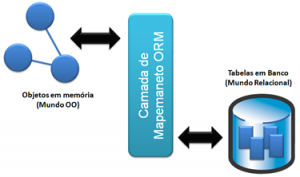
\includegraphics[scale=0.5]{imagens/orm.png}
\end{center}
Existem dois mundos: o relacional e o orientado a objetos, no mundo relacional prevalecem princípios matemáticos com a finalidade de armazenar e gerenciar corretamente os dados, de forma segura e se trabalha com a linguagem SQL que é utilizada para dizer o banco de dados “O QUE?” fazer e não como fazer.

Já no mundo orientado a objetos trabalhamos com classes e métodos, ou seja, se trabalha com fundamentados na engenharia de software e seus princípios que dizem “COMO” fazer. O ORM é justamente, a ponte entre estes dois mundos, ou seja, é ele quem vai permitir que a aplicação armazene os objetos no banco de dados. Para isto se faz necessário fazer um mapeamento dos seus objetos para as tabelas do banco de dados.
\begin{center}
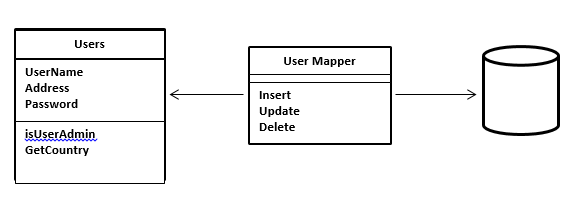
\includegraphics[scale=0.7]{imagens/work-orm.png}
\end{center}

A figura anterior traz uma ideia de como o ORM trabalha. Ele faz o mapeamento da sua classe para o banco de dados e cada ORM tem suas particularidades para gerar o SQL referente a inserção do objeto que corresponde a uma tabela no banco de dados e realizar a operação. Utilizando um ORM, também se ganha produtividade, pois deixa-se de escrever os comando SQL para deixar que o próprio ORM, faça isto por você. \cite{cadu_conceitos_2011}

\section{Astah}
O software foi desenvolvido no Japão na plataforma Java, o que garante sua portabilidade para qualquer plataforma que possui JVM (Máquina Virtual Java). JUDE (Ambiente para Desenvolvedores UML e Java) obteve o prêmio “Produto de Software do Ano 2006”, pela Agência de Promoção de Informação Tecnológica no Japão. Anteriormente conhecido como JUDE, ele funciona nas plataformas Windows, Mac e Linux. \cite{franco_neto_tutorial_2017}

Modelagem define os seus sistemas de uma forma que é mais fácil de entender, simples de comunicar e mais em contato com as pessoas que irão utilizar. Na área de Engenharia de Software, a UML (Linguagem de Modelagem Unificada) é uma linguagem de modelagem que permite representar um sistema de forma padronizada. Astah utilizada nos diagramas dinâmicos, essa ferramenta já é bastante consolidada, voltada para a modelagem de sistemas utilizando a UML, utiliza como recurso adicional a modelagem MAS ML (Modelagem de um Sistema Multiagente).

UML, criada por Grady Booch, Ivar Jacobson \& Jaimes Rumbaugh. É hoje o método mais comum para o paradigma orientado a objetos. Os objetivos da UML são: especificação, documentação, estruturação para sub-visualização e maior visualização lógica do desenvolvimento completo de um sistema de informação. UML 2.2, conforme a OMG (Object Management Group – organização internacional que aprova padrões abertos para aplicações orientadas a objetos), possui 14 tipos de diagramas, divididos em duas grandes categorias: Estruturais e Comportamentais. Sete tipos de diagramas representam informações estruturais, e os outros sete representam tipos gerais de comportamento, incluindo quatro em uma sub-categoria que representam diferentes aspectos de interação. Estes diagramas podem ser visualizados de forma hierárquica, como apresentado no padrão de diagrama de classes a seguir.

\begin{center}
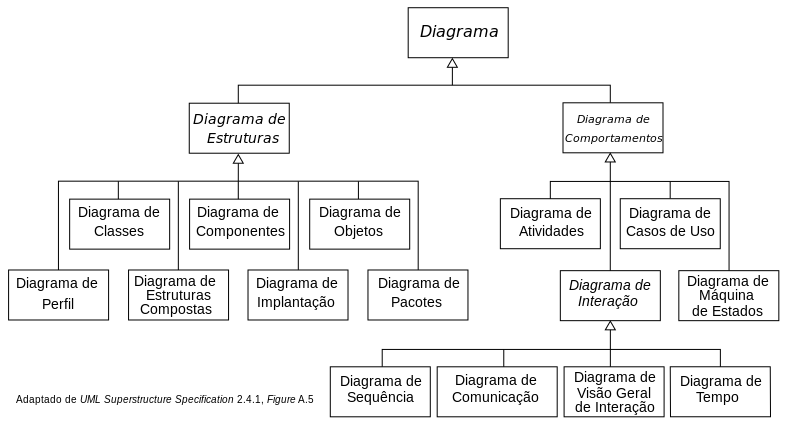
\includegraphics[scale=0.4]{imagens/UML_diagrams_overview_pt.svg_.png}
\end{center}

No Astah é possível modelar 9 dos 14 tipos de diagramas que são eles:

* Diagrama de Estruturas: Diagrama de Classes, Diagrama de Estruturas Compostas, Diagrama de Componentes e Diagrama de Implantação.
* Diagrama de Comportamentos: Diagrama de Atividades, Diagrama de Interação, Diagrama de Casos de Uso e Diagrama de Máquina de Estados.
* Diagrama de Interação : Diagrama de Sequência e Diagrama de Comunicação.

\section{Visual Studio Code}
Em 2015, a Microsoft introduziu um editor de código para desenvolver aplicativos da Web chamado Visual Studio Code, ou \citeonline{vscode}, abreviado. Anunciado durante o Build, um evento anual para desenvolvedores nos EUA, é uma ferramenta leve e multiplataforma disponível para Windows, Mac OS e Linux e atende a uma ampla variedade de projetos, não apenas ASP. .NET e Node.js. Além disso, o editor suporta a sintaxe de Python, Ruby, C++ e outras linguagens.

Além de ser totalmente gratuito, na segunda metade do lançamento, durante o evento Connect(), o editor foi anunciado como open source, e o código está disponível no GitHub, o que permite que a comunidade técnica desenvolva e contribua com seu desenvolvimento e facilitar a criação de extensões e novas funcionalidades.

O VS Code sera utilizado em todo o processo de desenvolvimento, tanto na parte do front-end quanto na parte \citeonline{front-end}, e é uma ferramenta muito importante para entrega de aplicativos.